\section{System Overview}
\label{sec:system}

\begin{figure}
\centering
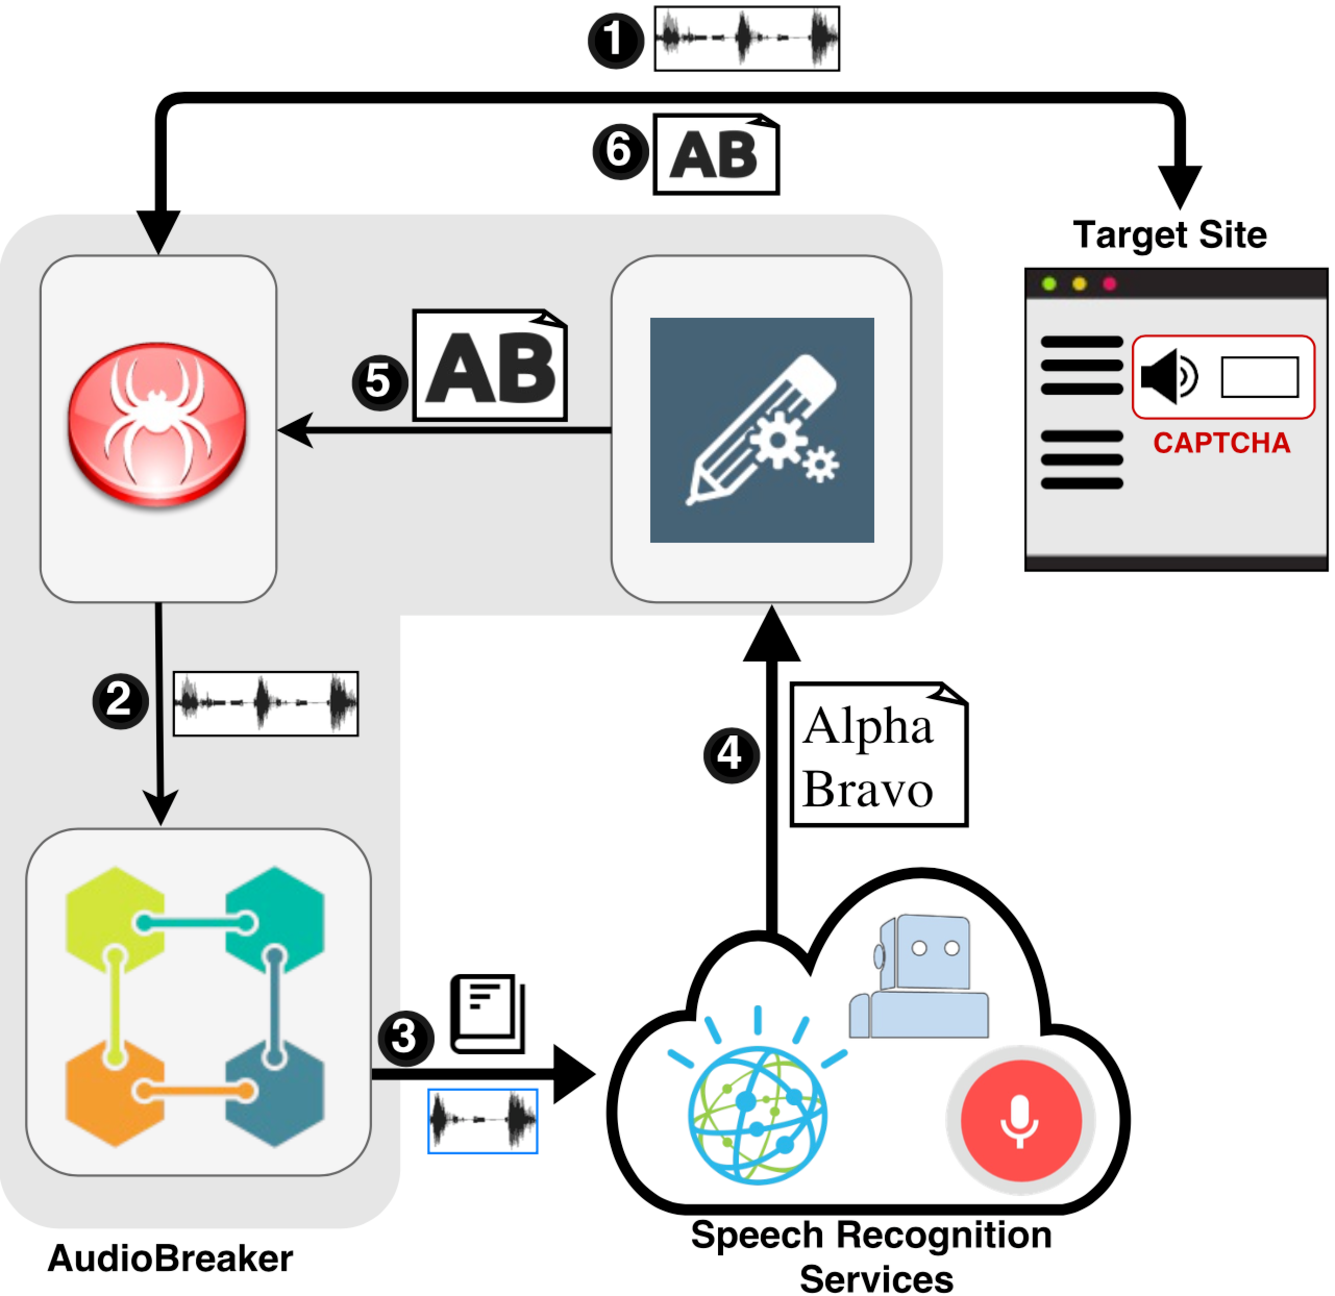
\includegraphics[width=\columnwidth]{figures/breaker_arch.pdf}
\caption{Overview of the CaptchaBreaker system.}
\label{fig:breaker}
\end{figure}

Describe our modular system. What components, how they have been implemented, how we create modules for each captcha service, and each speech recognition service.


We built a series of selenium bots that loads each service, obtains the audio file from the captcha for solving via the off the shelf voice recognition service. After the data is received it is post processed and specialzed for each serivce 


\subsection{Background on Selenium} 

To create the bot we utilized the browser automation framework known as selenium. This was the tool of our choice as it is hard to detect scraping/botting written utilizing the selenium webdriver and your browser of choice. Selenium communicates with browsers via a special protocol native to each browser and has access to everything loaded for a web site, the JavaScript, the DOM and even the secure cookies. The special protocol is required as  Selenium RC uses generic javascript for browser automation however executing simply generic javascript violates same origin policy. For every website the browser creates a sandbox for the website's javascript, this way the javascript that belongs to one website does not execute on another website that is currently loaded on the browser. (more detail on cross site scripting). To overcome this Selenium acts as an HTTP Proxy server, when we launch the browser through selenium scripts, javascript (Selenium Core) is injected into the browser, all subsequents requests are therefore through Selenium. In essence selenium makes the browser think that the web application is served from Selenium's domain rather than the actual web server hosting our web application.   

Selenium driving the browser from within by sitting in as injected Javascript provides certian limitations which is handled by "WebDriver" an object oriented api, as the Core is limited by the JavaScript sandbox of the browser (Due to same origin policy). The Webdriver, handles the browser from outside the browser. This was the marked difference between Selenium 1.0 and Selenium 2.0 as by being limited by the sandbox and therefore has reduced functional test coverage. 


[graphic of selenium driving browsers with injected javascript]


\subsection{Why Selenium}

\note{Why selenium is better than other botting/scrapers out there --
}

Almost no way to detect the automation except for checking some predefined variables which most websites do not do.

\note{source : https://stackoverflow.com/a/41220267
}

Web Driver is the nearest you can get to an actual person driving the browser automation. Quote:  "Driving a browser natively as a user would either locally or on a remote machine using the Selenium Server it marks a leap forward in terms of browser automation."

\note{source: http://www.seleniumhq.org/projects/webdriver/
}

\note{need better ways to say this}


We utilized three different voice recognition services for our system, the python google cloud speech api, the ibm bluemix, Wit ai voice recognition services.
